\chapter{Výsledky práce}

\section{Príklady kriviek}
Pri konštrukcií obálok elipsoidov sme vyriešili aj o rozmer nižší prípad, a to, obálku jednoparametrického systému elíps v rovine ležiacich na rovinnej krivke $m(t) \subset \mathbb{R}^2$. Pre rovinné prípady sme výsledky vizualizovali v online nástroji Desmos \cite{Desmos}, kde sme zadávali matematické výrazy vypočítané skriptom v Pythone \verb|2D_worklow.| V adresári sa nachádza niekoľko textových súborov s výpočtami.

\begin{example}[Parabola]
Majme parabolu s parametrizáciou $m(t)=(t, t^2).$ Na tejto krivke zostrojme jednoparametrický systém elíps so škálovaním v dotykovom smere krivky $a$ a v normálovom smere krivky $b$. 
%Vypočítajme derivácie krivky 
%\begin{align*}
%\dot{m}(t)&=(1, 2t) \\
%\| \dot{m} \|^2 &= 1+4t^2 \\
%\ddot{m}(t)&=(0, 2) \\
%\end{align*}
Jednoparametrický systém elíps má rovnicu
\begin{flalign*}
& Q \colon \quad \frac{1}{a^{2} b^{2}\left(4 t^{2} + 1\right)} \left( (x-t)^2 (b^2 + a^{2} 4t^2) + (y-t^2)^2 (a^2 + b^2 4t^2) \right) & \\
& + \frac{1}{a^{2} b^{2}\left(4 t^{2} + 1\right)} \left( 4t(b^2 - a^2)(x-t)(y-t^2)2t \right) - 1 = 0.
\end{flalign*}
Koeficienty derivácie $\dot{Q}$ 
\begin{flalign*}
& \dot{A}  = \frac{8 t \left(a^{2} - b^{2}\right)}{a^{2} b^{2} \left(16 t^{4} + 8 t^{2} + 1\right)} & \\
& \frac{\dot{B}}{2} = \frac{2 (4 t^{2} - 1) (a^{2} - b^{2})}{a^{2} b^{2} \left(16 t^{4} + 8 t^{2} + 1\right)} \\
& \dot{C} = \frac{-8 t \left(a^{2} - b^{2}\right)}{a^{2} b^{2} \left(16 t^{4} + 8 t^{2} + 1\right)} & \\
& \frac{\dot{D}}{2} = \frac{ \left(- 8 a^{2} t^{4} - 6 a^{2} t^{2} - 8 b^{2} t^{4} - 2 b^{2} t^{2} - b^{2}\right)}{a^{2} b^{2} \left(16 t^{4} + 8 t^{2} + 1\right)} & \\
& \frac{\dot{E}}{2} = \frac{2 t \left(a^{2} - 16 b^{2} t^{4} - 8 b^{2} t^{2} - 2 b^{2}\right)}{a^{2} b^{2} \left(16 t^{4} + 8 t^{2} + 1\right)} & \\
& \dot{F} = \frac{2 t \left(4 a^{2} t^{4} + 2 a^{2} t^{2} + 32 b^{2} t^{6} + 28 b^{2} t^{4} + 8 b^{2} t^{2} + b^{2}\right)}{a^{2} b^{2} \left(16 t^{4} + 8 t^{2} + 1\right)}.
\end{flalign*}
Determinant 
$$
\Delta(t) = 0. 
$$
Subdeterminant
$$\Delta_{33}(t) = \frac{-4 (a^2 - b^2)^2}{a^{4} b^{4} \left(16 t^{4} + 8 t^{2} + 1\right)} < 0.$$
%po zjednodušení
%\begin{flalign*}
%& \dot{Q} \colon 8t(a^{2} - b^{2}) x^2 + 4(4 t^{2} - 1)(a^{2} - b^{2})xy - 8t(a^{2} - b^{2}) y^2 & \\
%& (- 16 a^{2} t^{4} - 12 a^{2} t^{2} - 16 b^{2} t^{4} - 4 b^{2} t^{2} - 2 b^{2})x + 4 t(a^{2} - 16 b^{2} t^{4} - 8 b^{2} t^{2} - 2 b^{2})y & \\
%& + 2t(4 a^{2} t^{4} + 2 a^{2} t^{2} + 32 b^{2} t^{6} + 28 b^{2} t^{4} + 8 b^{2} t^{2} + b^{2}) = 0. 
%\end{flalign*}
Rozklad na priamky $p(t)$ a $q(t)$ jednoparametrického systému $\dot{Q}$  
\begin{align*}
p(t)& \colon x+2ty - \left(t + 2t^{3}\right)=0, \\
q(t)& \colon -4tx+2y+2t^{2}-\frac{b^{2}\left(1+4t^{2}\right)^{2}}{b^{2}-a^{2}}=0.
\end{align*}
Krivosť krivky $m(t)$ je
\begin{align*}
\kappa(t) = \frac{2}{\left(1+4t^{2}\right)^{\frac{3}{2}}}.
\end{align*}
Pre $a=2$ a $b=1$ je $\lambda = \frac{1}{3}$.
$$
\kappa(t) > \frac{1}{3} \text{ pre } t \in (-0.759,0.759)
$$
Na tom intervale uvažujeme teda 4 prieniky.
\end{example}

\begin{figure}[h]
	\centering
	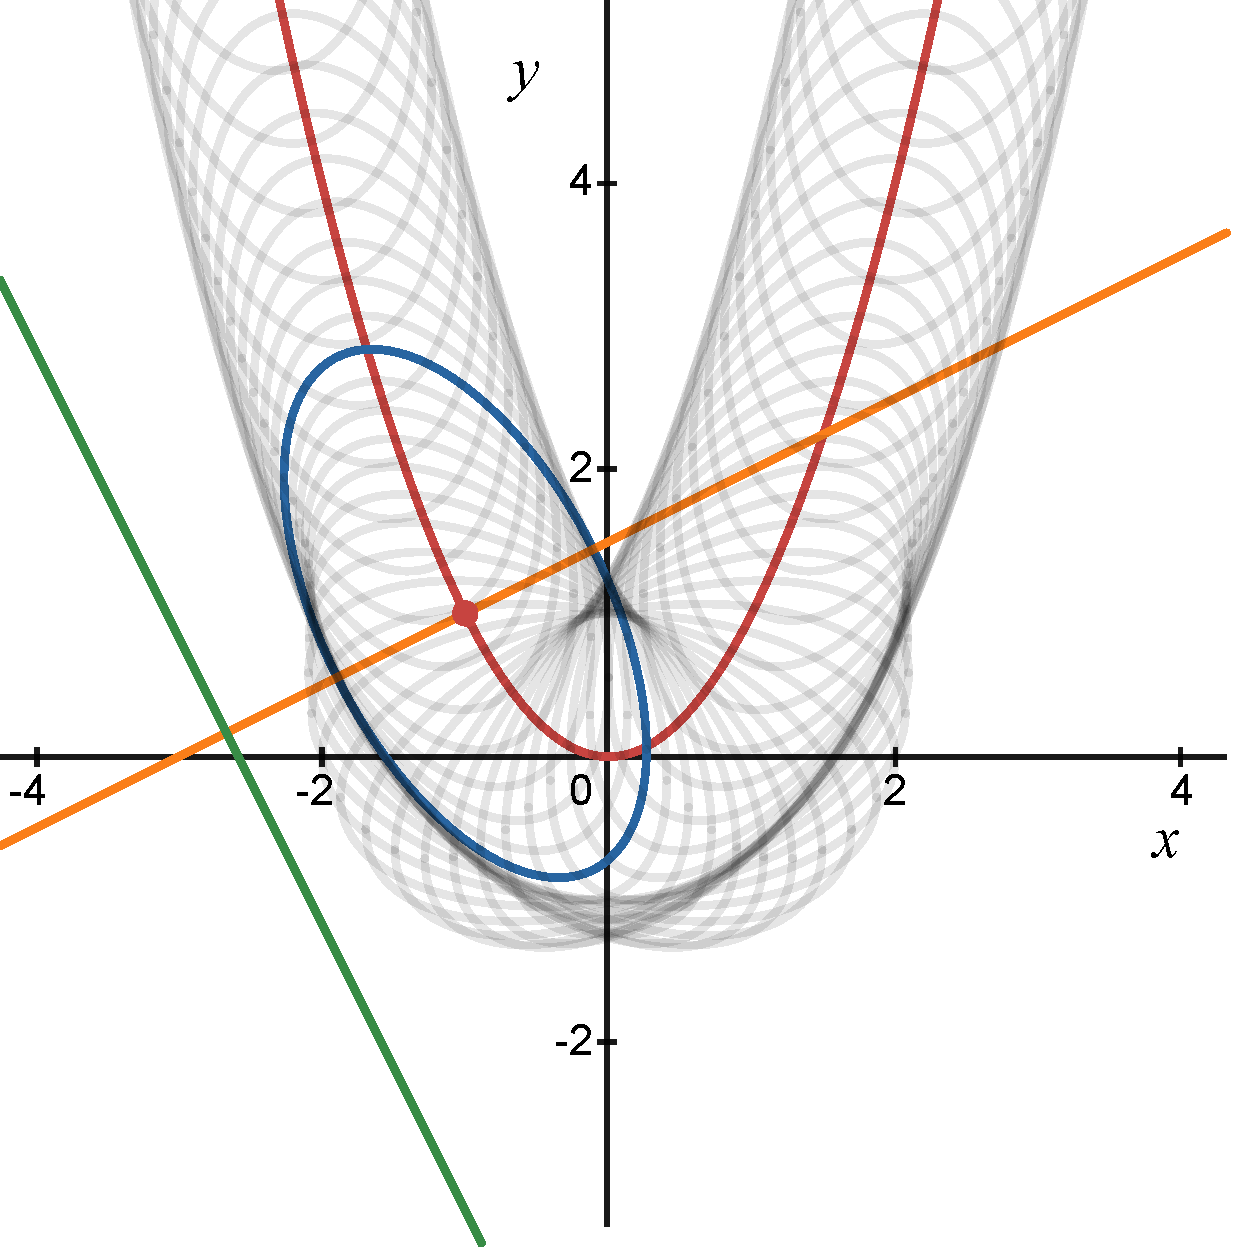
\includegraphics[width=0.5\textwidth]{images/parabola.pdf}
	\caption[Jednoparametrický systém na parabole.]{Jednoparametrický systém na parabole.}
	\label{fig:parabola}
\end{figure}

\section{Príklady plôch}
V tejto časti uvedieme pár vizualizácií, kde uvedieme aj parametre plôch.

\section{3D tlač}
Časti vytvorené z kružníc spojené automaticky generovaným meshom sme spojili s elipsoidmi a tak sme plochu mohli exportovať ako .stl súbor a pripraviť na 3D tlač cez PrusaSlicer uložením do formátu .gcode. S 3D tlačou bolo spojených niekoľko komplikácii. Pri prvých pokusoch sme zrejme použili nesprávnu kombináciu typu výplne, teda filamentu a rýchlosti tlačenia a teploty. 

\begin{figure}[h]
	\centering
	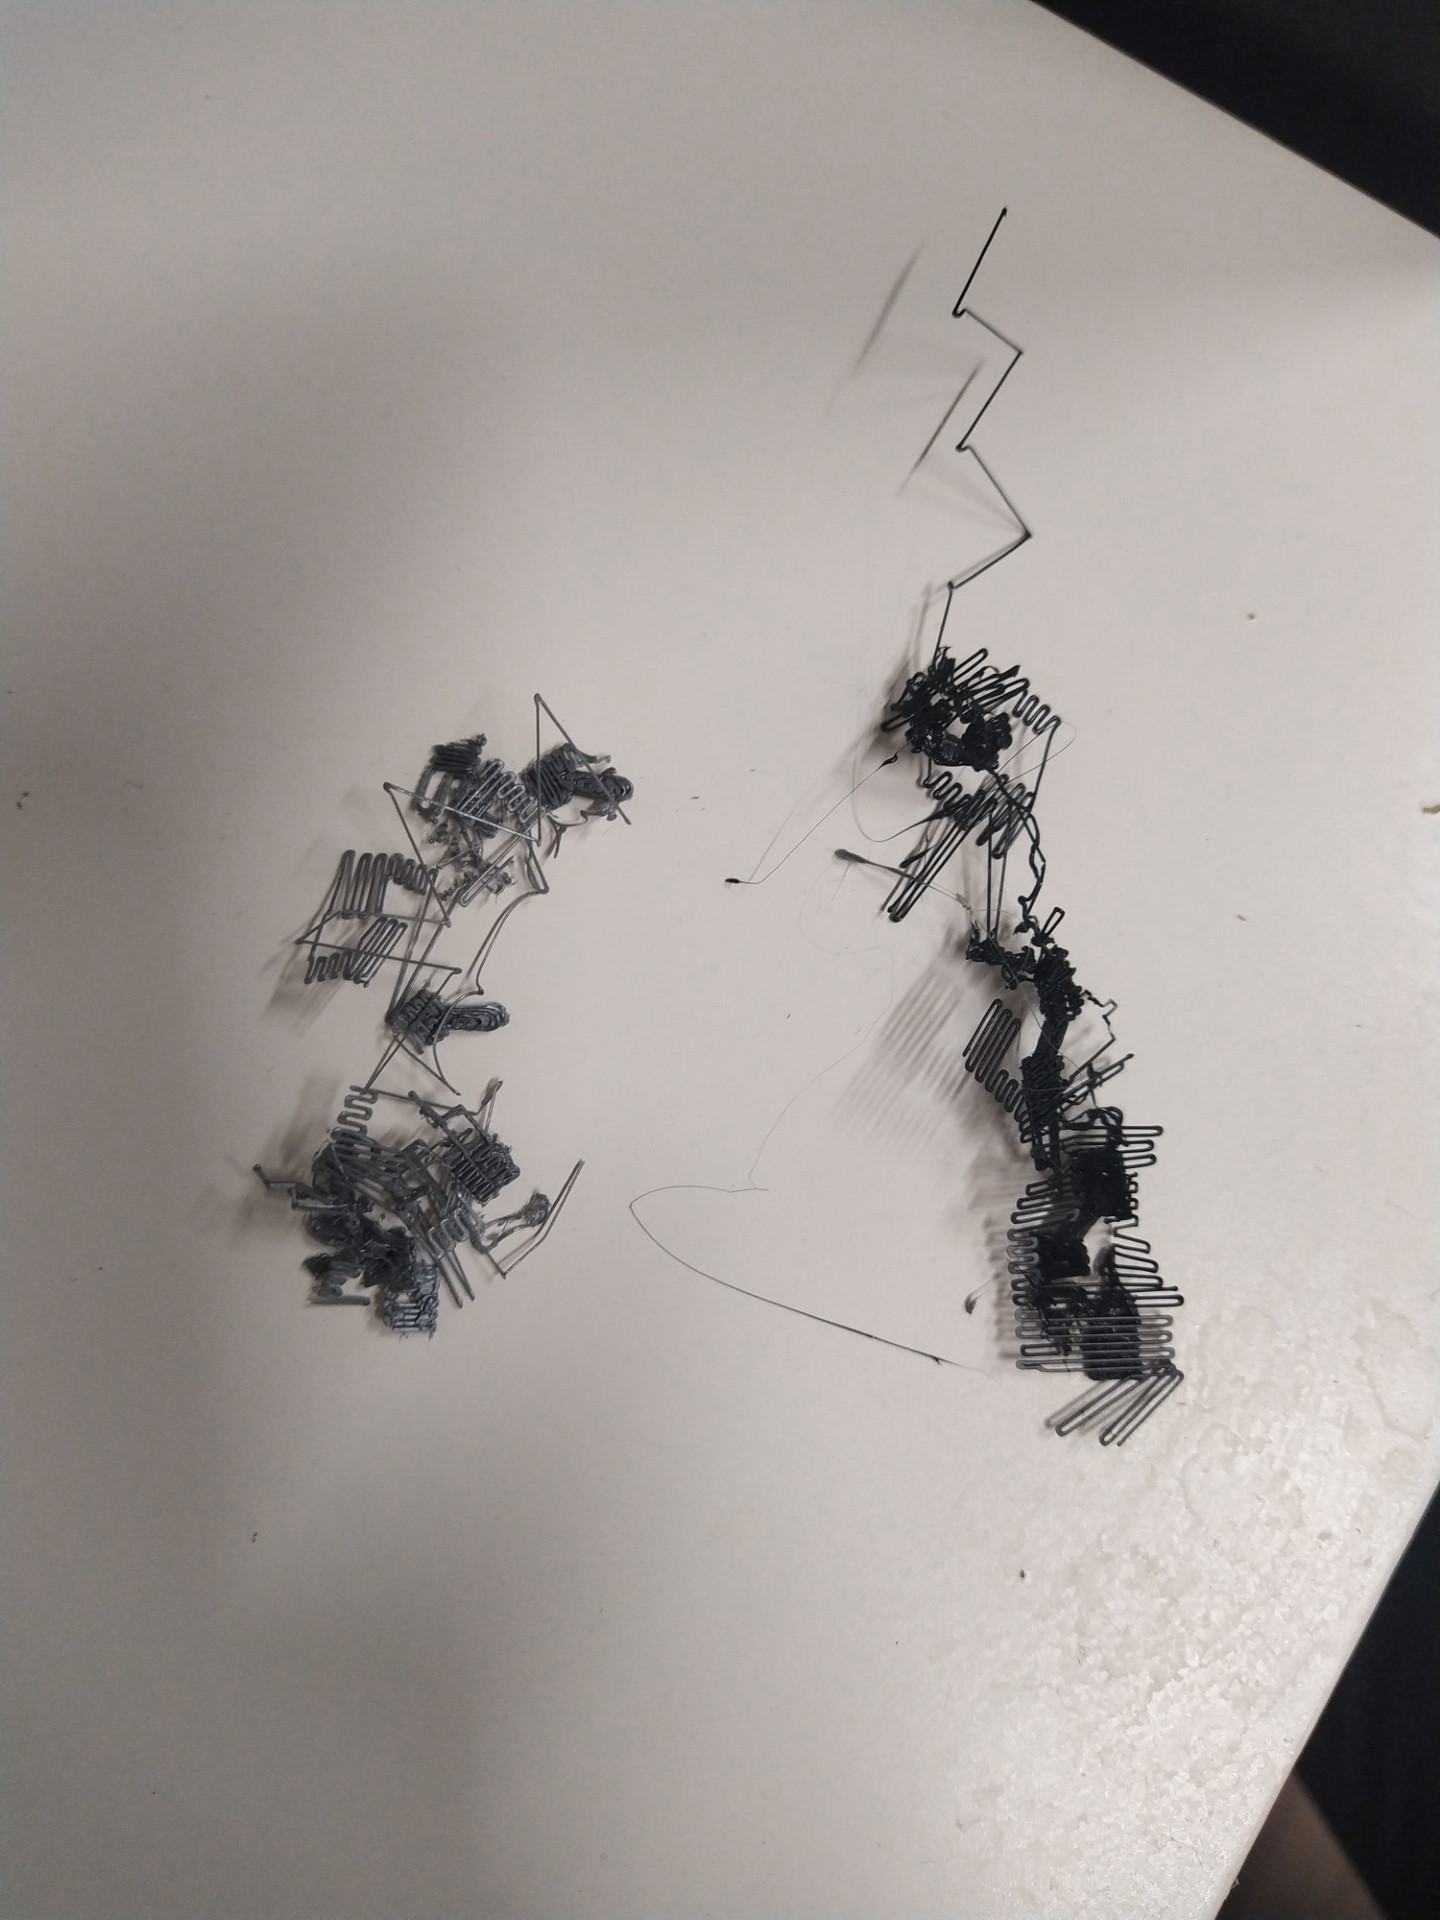
\includegraphics[width=0.5\textwidth]{images/tlac_prvy_pokus.jpg}
	\caption[Prvý pokus 3D tlače.]{Prvý pokus 3D tlače.}
	\label{fig:prvypokus}
\end{figure}

Neskôr tlačiareň odmietala tlač z SD karty, tak sme využili tlač z počítača pomocou softvéru Pronterface. Tlač z počítača bola mierne nepraktická, keďže musel byť celý čas zapnutý a pripojený k tlačiarni, ktorá nedisponovala káblom potrebnej dĺžky. Po niekoľkých úspešných výtlačkoch začala tlačiareň škrípať a bolo potrebné ju namazať a znova kalibrovať. Potom sme zistili, že tlačiareň podporuje tlač z SD karty, ktorá k nej bola dodaná a tlač už prebiehala pomerne bez problémov. Pri našej veľkosti plôch tlač trvala 90 až 150 minút. Plochy bolo potrebné škálovať, pretože boli príliš malé. Plochy bolo potrebné rôzne škálovať, príliš tenké časti by boli krehké. Použili sme škálovanie $500-750\%$. Vytlačili sme zopár prototypov a tri sady plôch, kde jedna sada obsahuje jednoparametrický systém sfér, obálku sfér, jednoparametrický systém elipsoidov a obálku elipsoidov. Po tlači sme ešte odstránili podporné štruktúry a tak sme dostali výsledné plochy. 

\begin{figure}[h]
	\centering	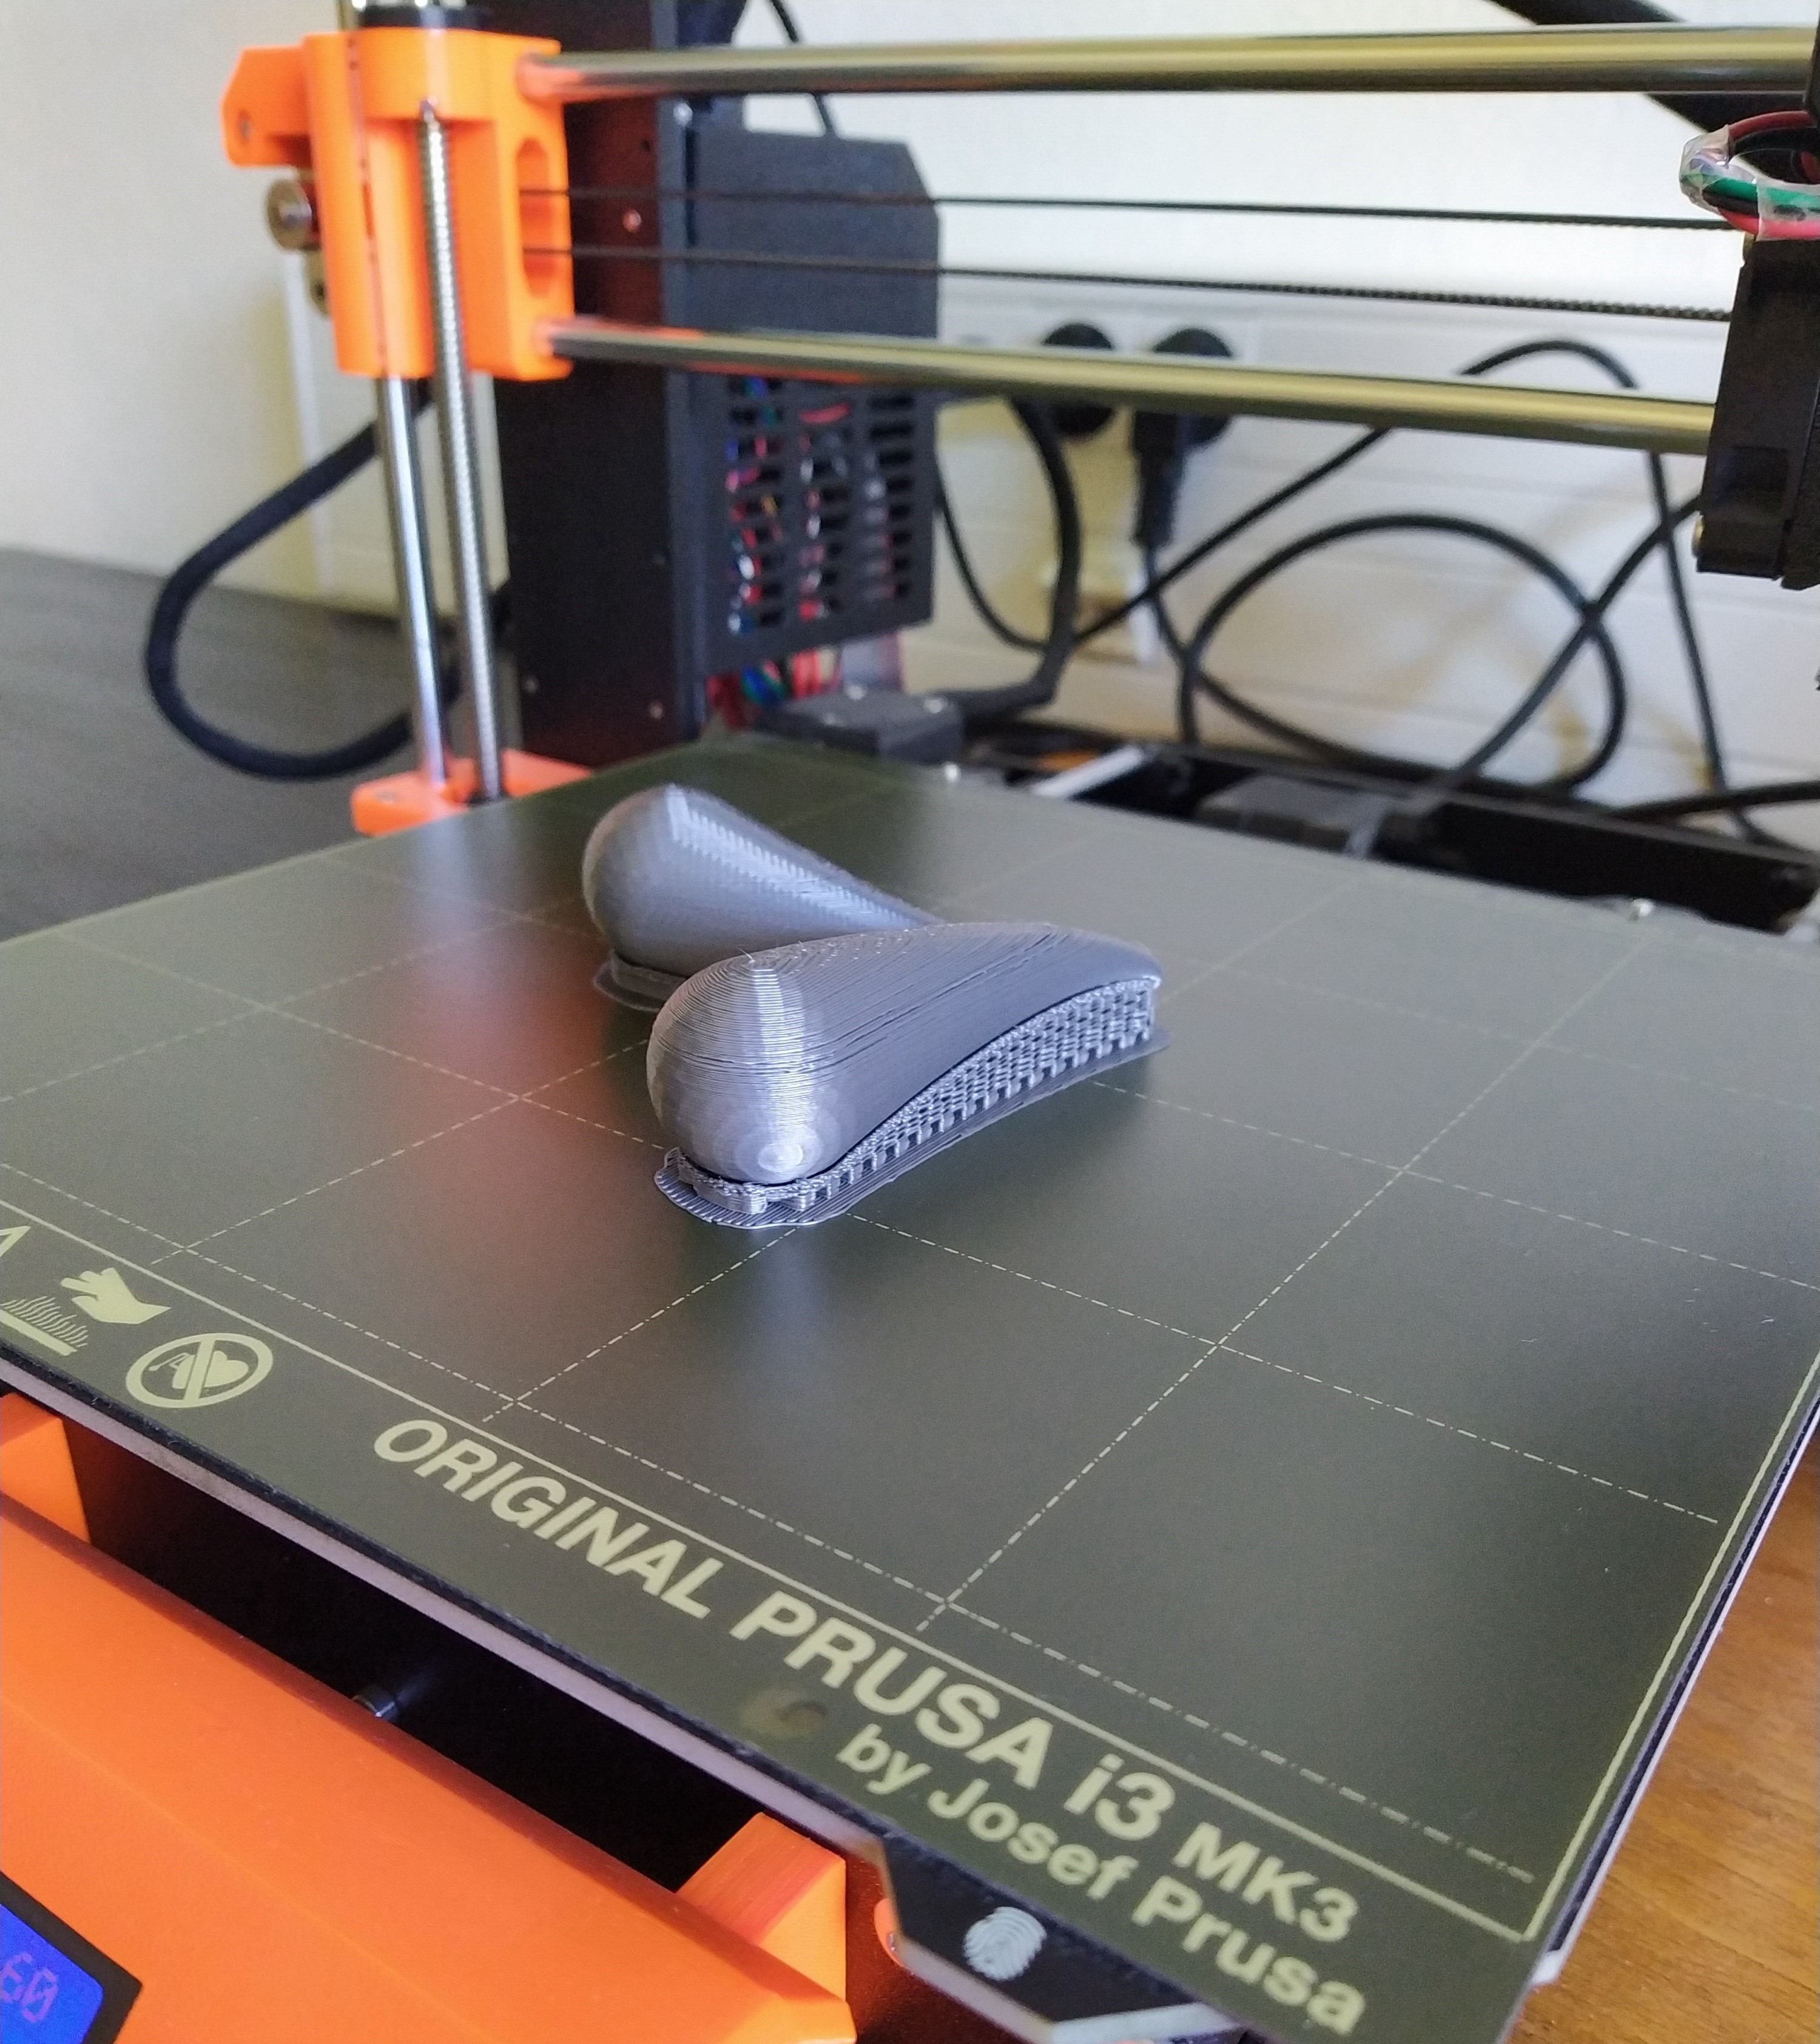
\includegraphics[angle=-90,width=0.5\textwidth]{images/plocha_v_tlaciarni.jpg}
	\caption[Plocha v 3D tlačiarni.]{Plocha v 3D tlačiarni.}
	\label{fig:plocha_v_tlaciarni}
\end{figure}

\section{Otvorené problémy}
Ak by sme chceli mať spájanie charakteristických kružníc plne automatizované, 
narazili by sme na niekoľko problémov. Na obr.~\ref{fig:spojenie_kruznic_1} sa pletivo medzi kružnice síce doplnilo očakávaným spôsobom, no v našom prípade to nesedí s požadovaným tvarom výslednej plochy.
Takisto sú výzvou uzavreté plochy a samoprieniky plôch ako na obr.~\ref{fig:spojenie_kruznic_2}.

\begin{figure}[h]
    \centering
    \begin{subfigure}[b]{0.6\textwidth}
        \centering
        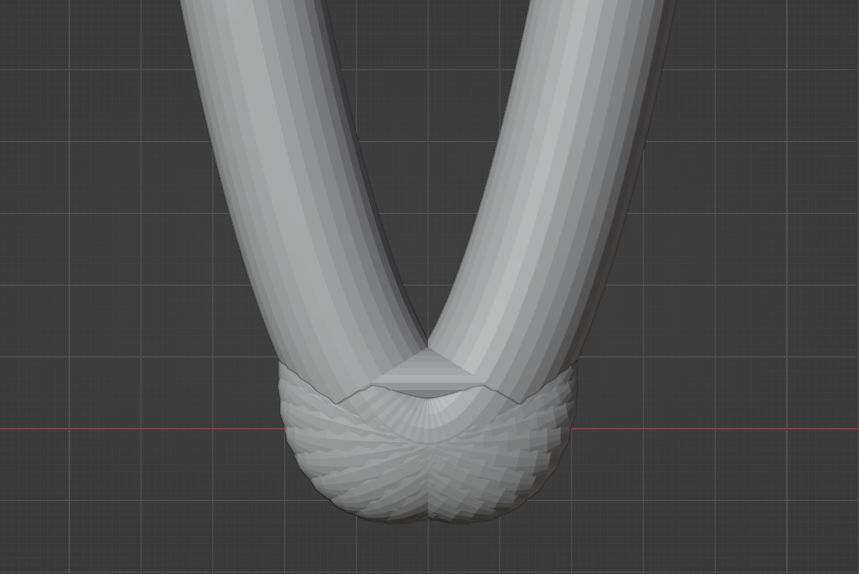
\includegraphics[width=\textwidth]{images/mesh.png}
		\caption[Spojenie kružníc.]{Spojenie kružníc.}
        \label{fig:spojenie_kruznic_1}
    \end{subfigure}
    \hfill
    \begin{subfigure}[b]{0.6\textwidth}
        \centering
        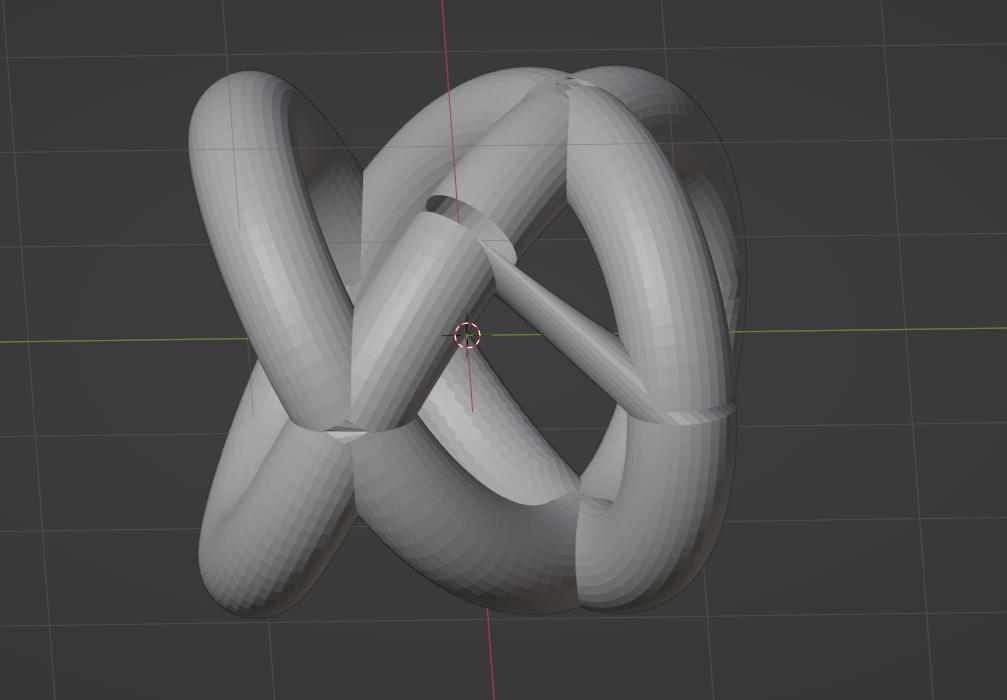
\includegraphics[width=\textwidth]{images/diery.png}
        	\caption[Uzavretá plocha so samoprienikmi.]{Uzavretá plocha so samoprienikmi.}
        \label{fig:spojenie_kruznic_2}
    \end{subfigure}
    	\caption[Doplnenie pletiva.]{Doplnenie pletiva.}
    \label{fig:spojenie_kruznic}
\end{figure}

%\begin{figure}[h]
%	\centering	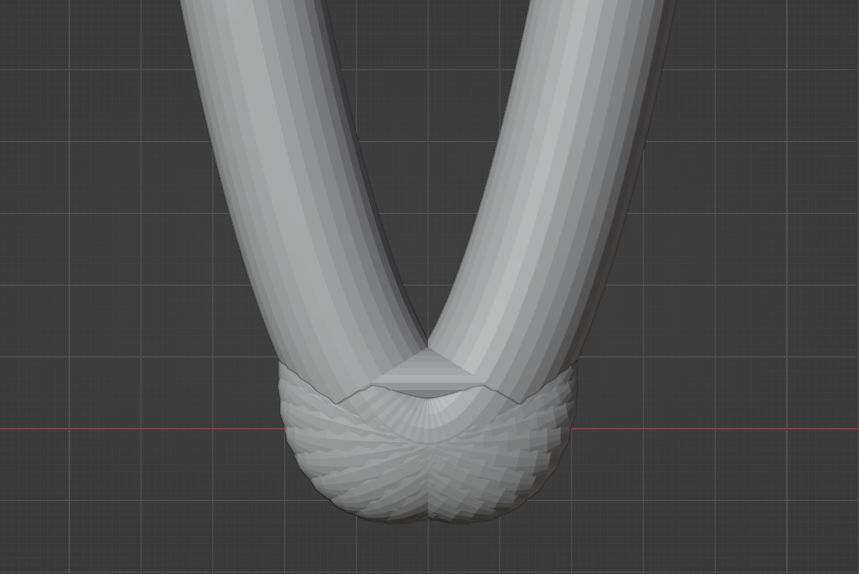
\includegraphics[width=0.5\textwidth]{images/mesh.png}
%	\caption[Spojenie kružníc.]{Spojenie kružníc.}
%	\label{fig:spojenie_kruznic}
%\end{figure}
%
%\begin{figure}[h]
%	\centering	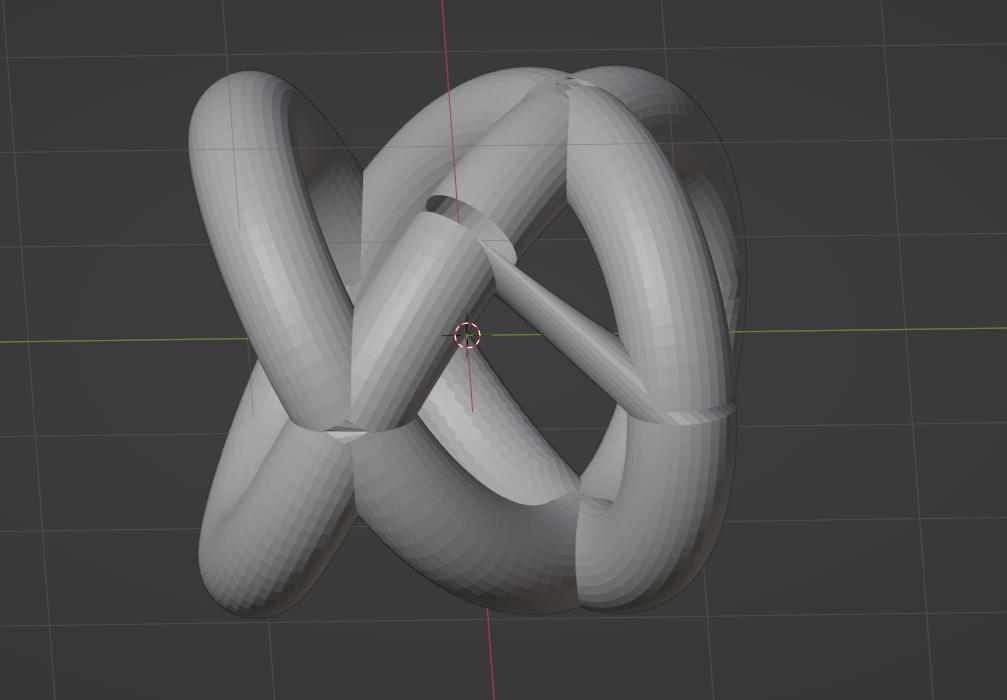
\includegraphics[width=0.5\textwidth]{images/diery.png}
%	\caption[Spojenie kružníc.]{Spojenie kružníc.}
%	\label{fig:spojenie_kruznic_2}
%\end{figure}

Ak by sme pre parametre $t,$ v ktorých $\kappa(t) > \lambda $ generovali charakteristickú elipsu a charakteristickú kružnicu namiesto elipsoidu, narazili by sme taktiež na problém vhodného spojenia týchto objektov a taktiež vygenerovaného pletiva.

\section{Budúca práca}
V budúcom výskume na matematickej úrovni môžeme uvažovať odlišný faktor škálovania $c \neq b$ v binormálovom smere $\vec{b}$ Frenetovho lokálneho súradnicového systému $(\vec{t}, \vec{n}, \vec{b})$ ku krivke $m(t)$. V tomto prípade by sme ako prienik roviny prechádzajúcej stredom elipsoidu nedostali charakteristickú kružnicu, ale elipsu.

Ďalším možným smerom rozšírenia práce je namiesto konštantného škálovania použiť funkcie škálovania $a(t), b(t),$ príp. $c(t)$, napríklad funkcie normy vektorov Frenetovho repéra, $a(t) = \| \vec{t} \|, b(t) = \| \vec{n} \| $ a $c(t) = \| \vec{b} \|$. 

Nasledujúcim krokom by mohlo byť upustenie od škálovania v jednotlivých smeroch Frenetovej bázy a škálovať jednoparametrocký systém elipsoidov ľubovoľne.

V implementačnej časti by pokračovanie predstavovalo zostrojenie obálky iba pomocou charakteristických kriviek, teda kružníc a elíps a taktiež vývoj plne automatického algoritmu na doplnenie pletiva medzi objektami. Tiež by mohla byť vytvorená aplikácia s interaktívnou možnosťou zmeny parametrov škálovania.